\section{Introduction}
Fluid dynamics is today a cornerstone to several fields of study, including ærospace engineering and meteorology.
Real world fluid behaviour is intricate and complex. Therefore, to gain insights into the governing principles of
fluid flow, simplified and idealised models are used. This essay investigates the application of vector calculus
to model and analyse steady, inviscid, and incompressible fluid flow in two-dimensional spaces around a circular
obstacle. These idealisations allow for the derivation of some of fluid dynamic's key mathematical formulæ and
provides a foundation for understanding less idealised fluids.

This essay will address the question: "\researchquestion" Through the derivation of the velocity potential and
vector field, this essay aims to demonstrate how fundamental laws of fluid motion can be expressed and used through
vector calculus.

% Aim & scope
\subsection{Aim \& scope}
The scope of this essay will be limited to the theoretical modelling of fluid flow in a two-dimensional space
as a vector field under idealised conditions forming steady, inviscid and incompressible fluid flow through the 
derivation of the velocity-potential. The analysis will be centred on the application of vector calculus to derive
fundamental formulæ and describe fluid behaviour around a stationary circular obstacle. Consequently, this essay
will not touch on viscous effects, turbulent flow or three-dimensional analysis, nor will it involve any experimental 
validation. The focus is on the mathematical derivation and analysis of the idealised model.

% Background
\subsection{Background}
\subsubsection{Glossary}
\begin{defn} % steady flow
    \definedterm{Steady flow} refers to flow in which the velocity at every point does not change over time \cite{CRACIUNOIU2001559}.
\end{defn}
\begin{defn} % inviscid flow
    \definedterm{Inviscid flow} is the flow of a fluid with 0 viscosity \cite{ANDERSON20031}.
\end{defn}
\begin{defn} % incompressible fluid
    An \definedterm{incompressible fluid} is a fluid whose density at every point does not change over time \cite{AHMED2019331}.
\end{defn}
\begin{defn} % scalar field
	A \definedterm{scalar field} is a function mapping points in space to scalar quantities such as temperatures.

	\begin{figure*}[!ht]
		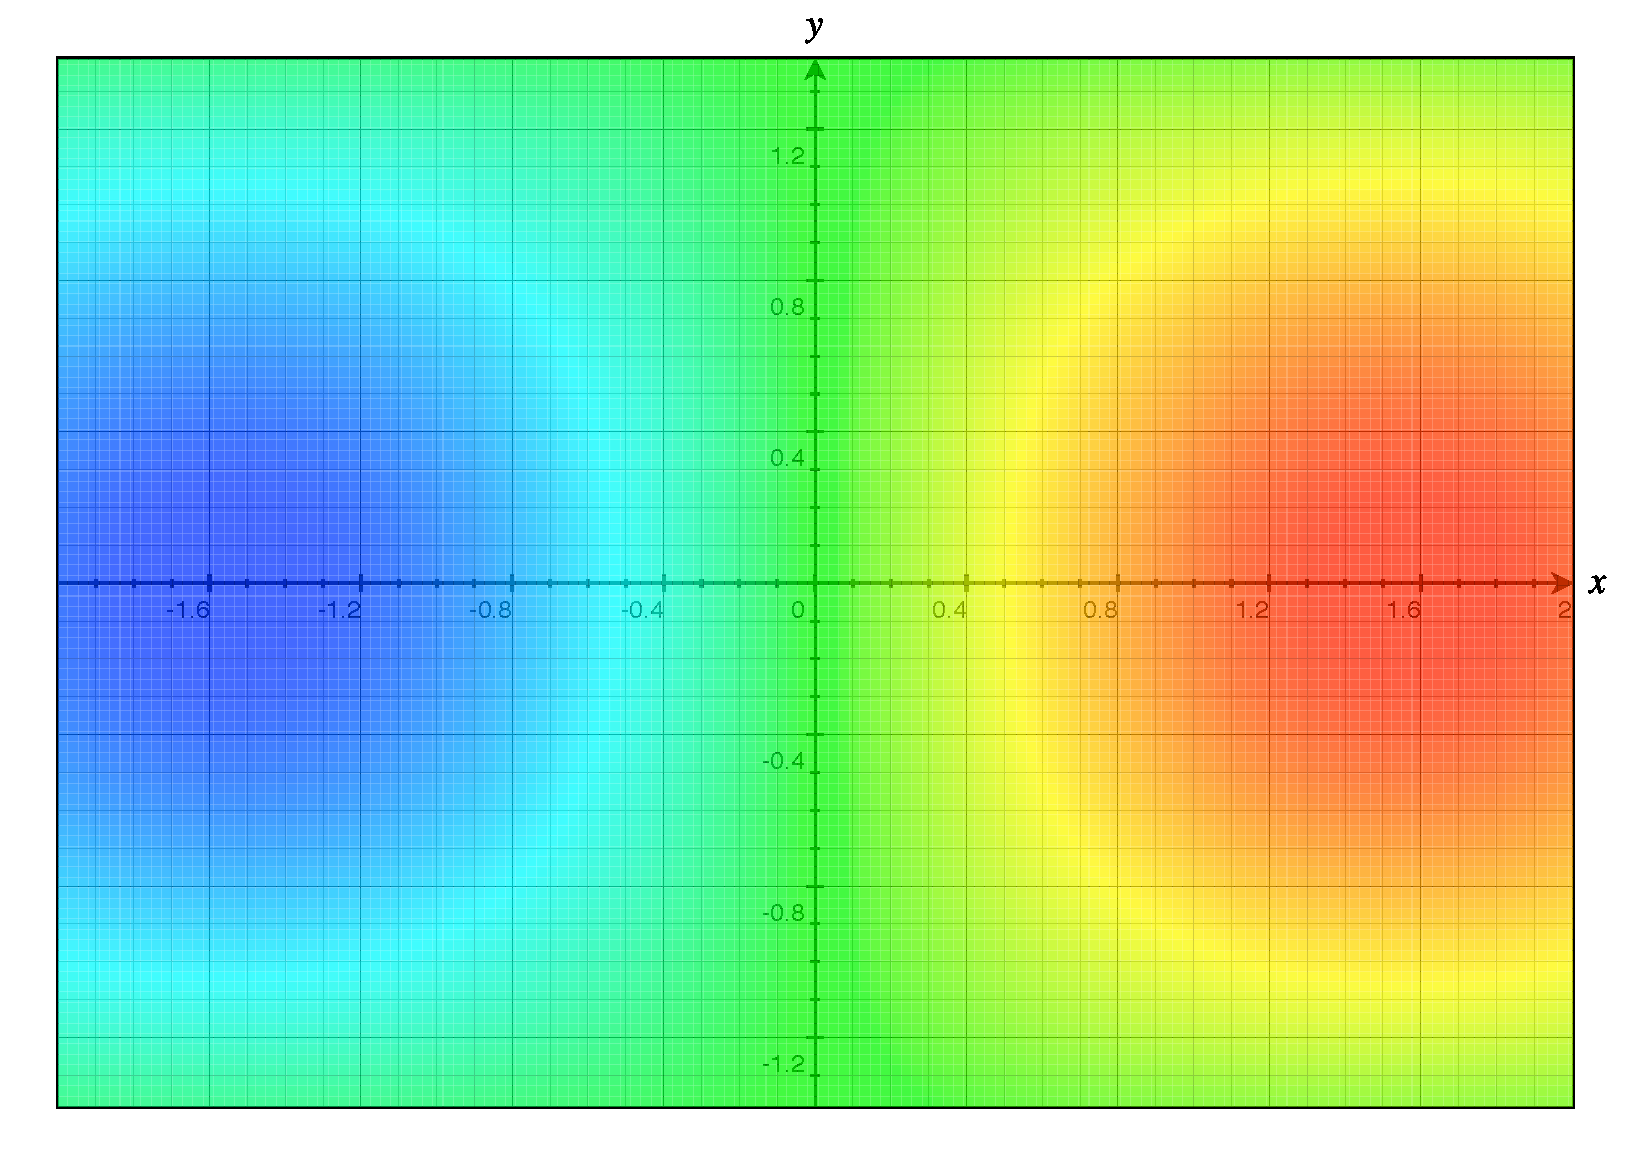
\includegraphics[scale=0.5]{scalar_field_example.pdf}
		\centering
		\caption{Scalar field plotted for the function $f(x,y)=\sin(x)\cos y$}
	\end{figure*}
\end{defn}
\begin{defn} % vector field
    A \definedterm{vector field} is a function mapping points in space to vector quantities \cite{BREZINSKI20063}. In
	the case of fluid dynamics, vector fields often model quantities like fluid velocity.

	\begin{figure*}[!ht]
		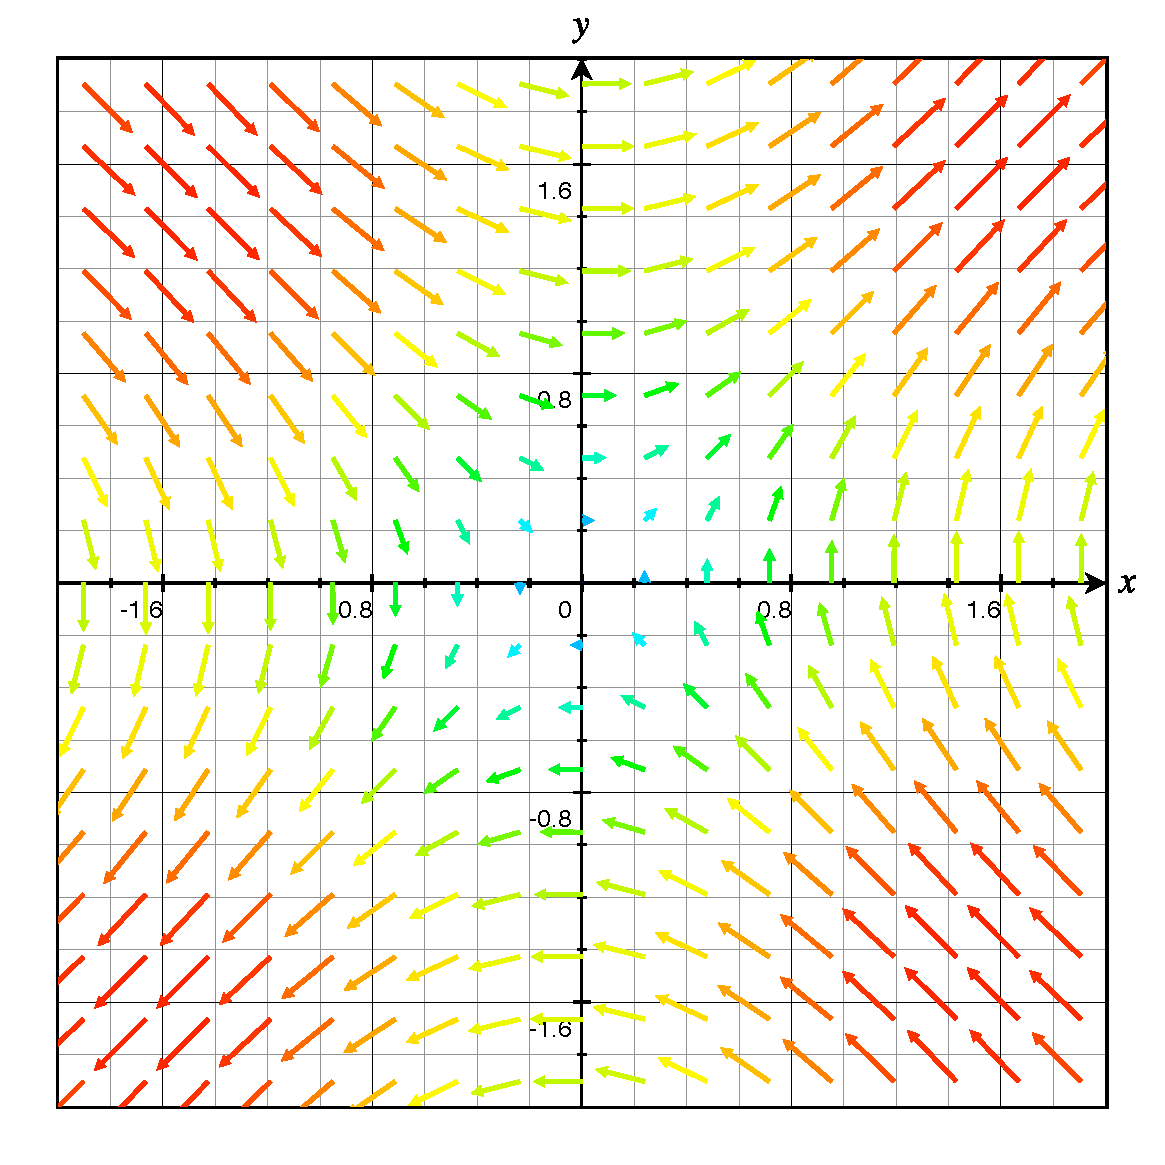
\includegraphics[scale=0.5]{vector_field_example.pdf}
		\centering
		\caption{Vector field plotted for the function $f(x,y)=\begin{pmatrix}
			\sin y\\\sin x
		\end{pmatrix}$}
	\end{figure*}
\end{defn}
\begin{defn} % velocity potential
	The \definedterm{velocity potential} $\phi$ is a scalar field whose gradient is the velocity vector field of some
	fluid, mathematically $\mathbf{V}=\nabla\phi$. The quantity is defined for irrotational flow which is a resulting
	property of the idealisations made in this essay\referto{theorem:kelvin}.
\end{defn}

\subsubsection{Notation}
Vector calculus, like one-variable calculus, has no standardized notation. This essay will employ the following
notation:
\begin{itemize}
	\item $\nabla$:
	\begin{itemize}
		\item $\gradient{F}$: The gradient of some scalar field $F$.
		\item $\divergence{\fatf}$: The divergence of some vector field $\fatf$.
		\item $\curl{\fatf}$: The curl of some vector field $\fatf$.
		\item $\nabla_\vec{v}f$: The directional derivative of $f$ in the direction of some vector $\vec{v}$
	\end{itemize}
	\item $\Delta$: The Laplacian operator
	\item $\disk{x}{y}$: The set of the points in an open disk centred at $\point{x}{y}$ with radius $\delta$
	\item $\ni$: "Such that"
	\item $\ihat\,\&\,\jhat$: Unit vectors in the positive $x$ and $y$ directions respectively.
	\item $\rhat\,\&\,\thetahat$: Unit vectors in the positive $r$ and $\theta$ directions respectively.
\end{itemize}

\subsection{The mean value theorem}
\begin{lemma}[Rolle's theorem]\label{lemma:ROLLES}
	If a function $f$ is continuous on the interval $[a,b]$ and differentiable on $(a,b)$, and $f(a)=f(b)$, then $\exists\,c\in(a,b)\ni f'(c)=0$.
	\begin{proof}
		If $\forall x\in(a,b), f(x)=f(a)=f(b)$, then trivially $f'(x)=0$. However, if 
		$f(x)\neq f(a)\,\forall x\in(a,b)$, then the value of $f$ must increase or decrease somewhere
		on the interval $(a,b)$. Consequently, there must exist a local extrema $\eta\in(a,b)$. Assume $\eta$ is a
		local maxima. Then consider the interval $I=(\eta-\delta,\eta+\delta)$ for some $\delta>0\ni\forall X\in I,f(X)\leq f(\eta)$.

		Let $h<0$ be a number sufficiently small such that $\eta-h\in I$. $f(\eta+h)\leq f(\eta)\implies f(\eta+h)-f(\eta)\leq0$. Thus,
		$$
			\frac{f(\eta+h)-f(\eta)}{h}\geq0\because\left\{\begin{matrix}
				f(\eta+h)-f(\eta)&\leq0\\
				h&\leq0
			\end{matrix}\right.
		$$
		Taking the left-hand limit as $h\rightarrow0$,
		$$
			\lim_{h\rightarrow0^-}\frac{f(\eta+h)-f(\eta)}{h}=f'(\eta)
		$$
		Now let $H>0$ be a number sufficiently small such that $\eta-H\in I$.
		\begin{align*}
			\frac{f(\eta+H)-f(\eta)}{H}&\leq0\because\left\{\begin{matrix}
				f(\eta+H)-f(\eta)&\leq0\\
				H&\geq0
			\end{matrix}\right.\\
			\lim_{H\rightarrow0^+}\frac{f(\eta+H)-f(\eta)}{H}&=f'(\eta)
		\end{align*}
		Thus,
		\begin{align*}
			0\geq\lim_{H\rightarrow0^+}\frac{f(\eta+H)-f(\eta)}{H}=&f'(\eta)=\lim_{h\rightarrow0^-}\frac{f(\eta+h)-f(\eta)}{h}\geq0\\
			\therefore\,&f'(\eta)=0
		\end{align*}
		Since the same would apply for local minima, then for any local extrema $c\in(a,b),f'(c)=0$
	\end{proof}
\end{lemma}
\begin{lemma}[The mean value theorem]\label{lemma:MVT}
	For any function $f$ continuous on the interval $[a,b]$ and differentiable on the interval $(a,b)$,
	$\exists\,c\in(a,b)\ni$
	\begin{equation}\label{equation:MVT}
		f'(c)=\frac{f(b)-f(a)}{b-a}
	\end{equation}
	\begin{proof}
		Let the vector $\vec{v}$ represent the vector from $\point{a}{f(a)}$ to $\point{b}{f(b)}$.
		$$
			\vec{v}=\begin{bmatrix}
				b-a\\
				f(b)-f(a)
			\end{bmatrix}
		$$
		Then let the vector $\vec{\hat{n}}$ represent a vector normal to the curve of $f$ at any point $c\in(a,b)$.
		The angle between the $x$-axis and $f'(c)$ is $\atan f'(c)$. Thus, $\vec{\hat{n}}$ can be expressed as:
		$$
			\vec{\hat{n}}=\begin{bmatrix}
				-\sin\atan f'(c)\\
				\cos\atan f'(c)
			\end{bmatrix}
		$$
		If point $c$ satisfies \eqref{equation:MVT}, then $\vec{\hat{n}}\cdot\vec{v}=0$.
	\end{proof}
\end{lemma}

% \begin{tikzpicture}
% \begin{axis}[
% title={$x \exp(-x^2-y^2)$},
% domain=-2:2,
% view={0}{90},
% colormap/viridis,
% colorbar,
% ]
% \addplot3[
%     surf,
% 	shader=interp,
% 	samples=20
% ]
% { sin(deg(x))*cos(deg(y)) };
% \end{axis}
% \end{tikzpicture}